%!TEX encoding = UTF-8 Unicode
%!TEX program = xelatex
%% This template licensed under CC-BY-NC-SA by Koenraad De Smedt
\documentclass[final, fmstyle, 12pt]{article}
\usepackage[utf8]{inputenc}
%\usepackage[spanish]{babel}
\usepackage[margin=24mm]{geometry}
\usepackage{fontspec,xltxtra,polyglossia,titling,graphicx,dingbat}
\usepackage{verbatim,gb4e,synttree,multicol} % choose or add what you need   
\usepackage[colorlinks,urlcolor=blue,citecolor=black,linkcolor=black]{hyperref}
\setmainfont[Mapping=tex-text]{Times New Roman} % or another similar font
\setdefaultlanguage{spanish}
%\setotherlanguages{english}
\usepackage[numbers]{natbib}
\usepackage{xspace}
\usepackage{float}
\usepackage{dirtytalk}
\usepackage{subfiles}
\usepackage{graphicx}
\hypersetup{
    colorlinks=true,
    linkcolor=black,
    filecolor=magenta,      
    urlcolor=black,
    pdftitle={Memoria experiencia profesional},
    pdfpagemode=FullScreen,
    }
\urlstyle{same}
\frenchspacing
%\newcommand{\checkmark}{x}

\title{MEMORIA DE EXPERIENCIA PROFESIONAL GRUPO TOMZA}
\author{Héctor Hugo Vidaña Arrieta}
\date{\today}
\hyphenation{unicode}
\usepackage{url}
\usepackage{hyperref}
%\usepackage[bitstream-charter]{mathdesign}
\begin{document}
\renewcommand{\tablename}{Tabla}
	\thispagestyle{empty}
\begin{center} \vfill
{\Large UNIVERSIDAD AUTÓNOMA DE CIUDAD JUÁREZ}\\
\vspace{6mm}
{\large Instituto de Ingeniería y Tecnología\\
\vspace{6mm}
Departamento de Ingeniería Eléctrica y Computación
\vspace{20mm}


\includegraphics [scale=0.7]{Imagenes/escudo-uacj} 
\vspace{10mm}


\thetitle\\
\vspace{15mm}

Protocolo de investigación presentado por:\\
\vspace{6mm}
\theauthor\hspace{10mm} 159957\\
\vspace{10mm}
Requisito para la obtención del título de\\
\vspace{6mm}
INGENIERO EN SOFTWARE\\
\vspace{10mm}

Asesora:\\
{Dra. Julia Patricia Sánchez Solis}\\
} \vfill
	Ciudad Juárez, Chihuahua \hspace{70mm}\today

% {\small \href{https://creativecommons.org/licenses/by/4.0/}{\includegraphics[height=1.2em]{cc-by}} by \theauthor}
\clearpage

\end{center}

\newpage
\begin{center}

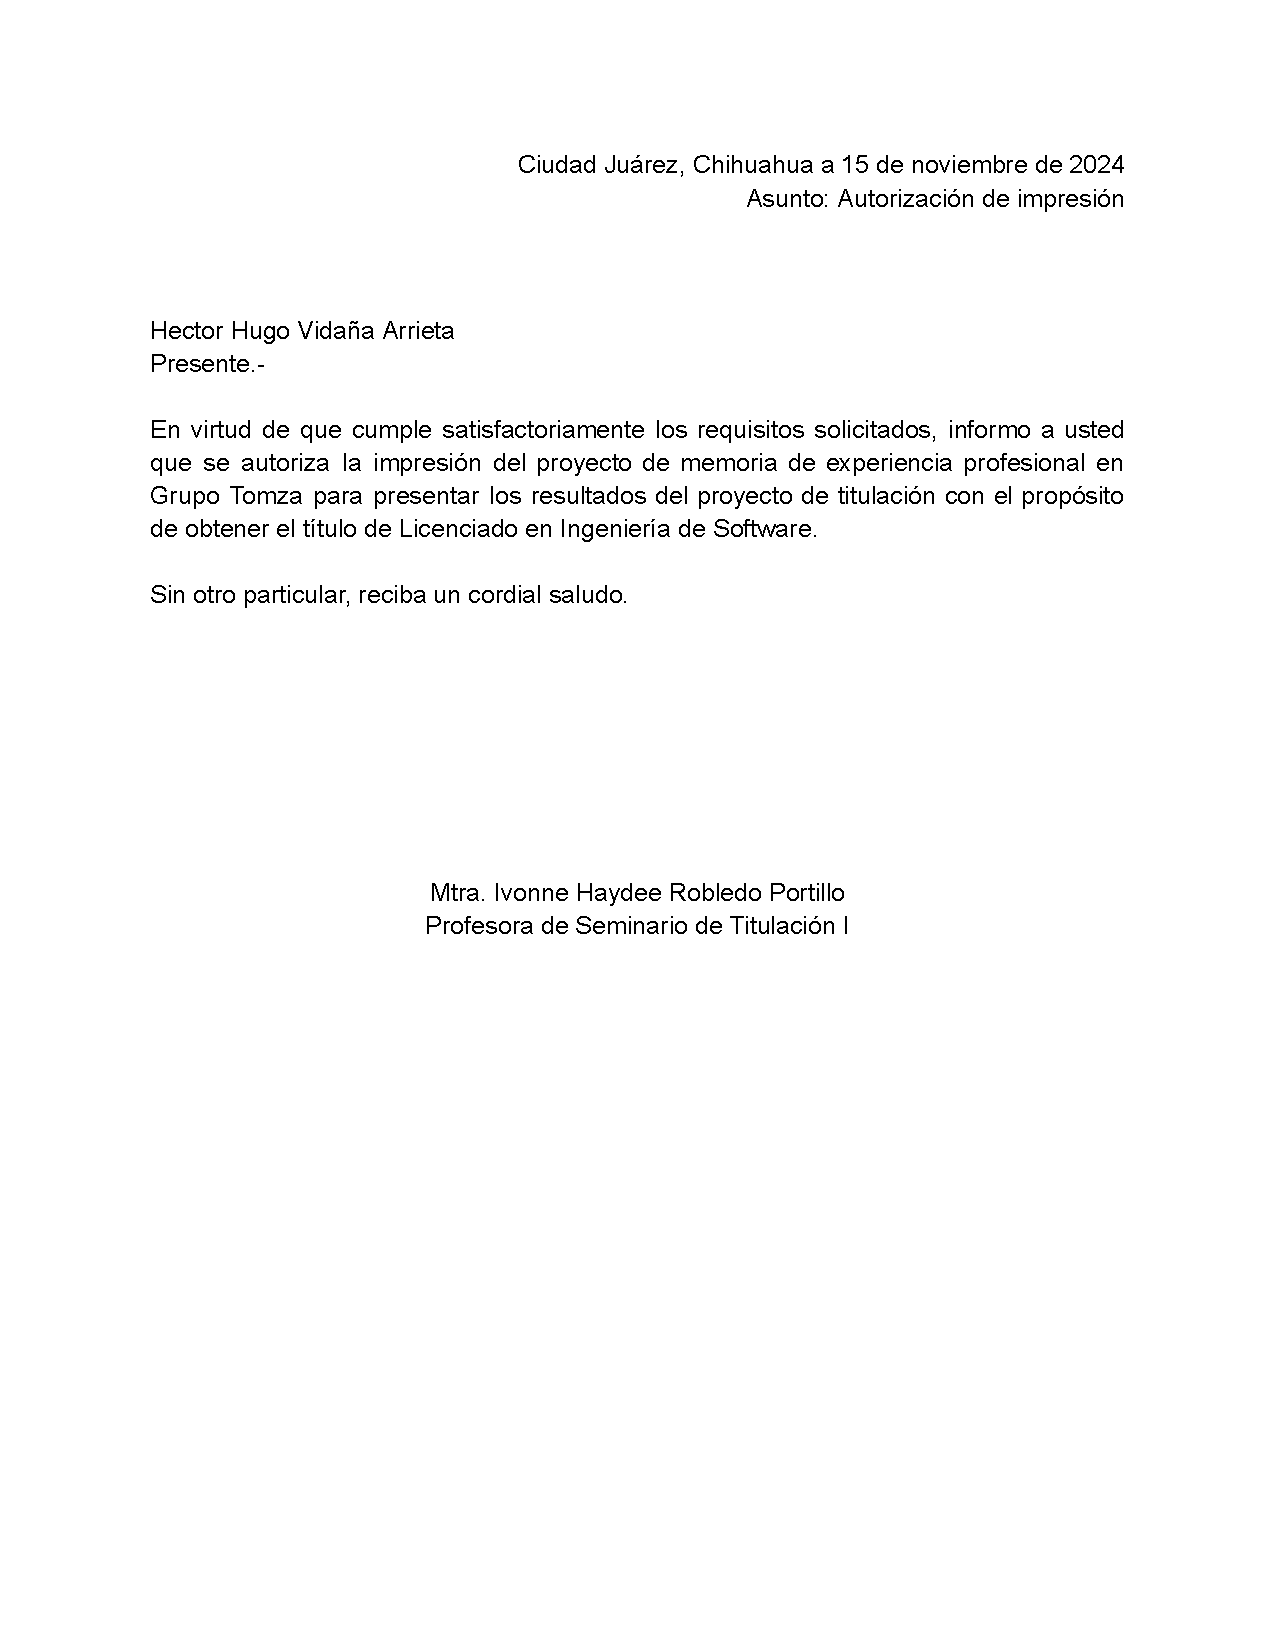
\includegraphics[scale=0.8]{Imagenes/Pdf/Carta de maestro.pdf}
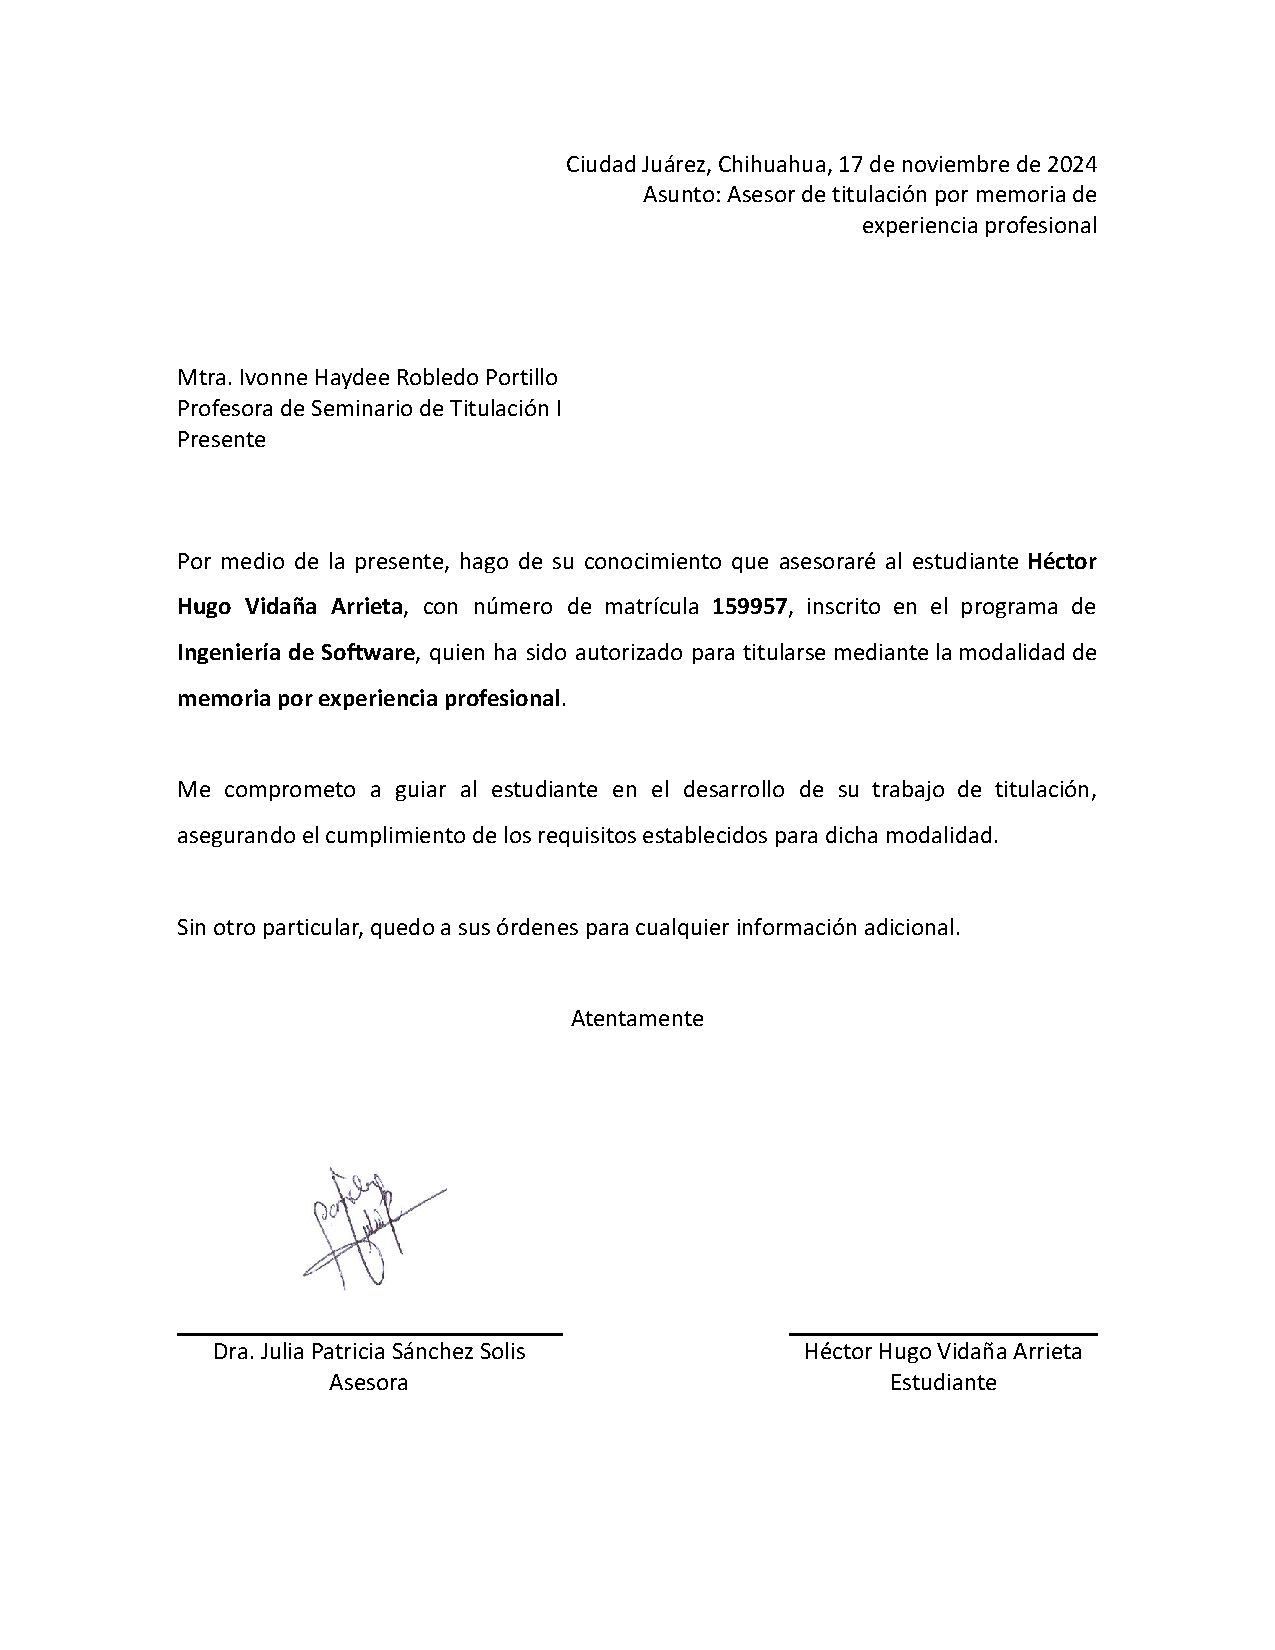
\includegraphics[scale=0.8]{Imagenes/Pdf/Carta asesor.pdf}
\includegraphics[scale=0.8]{Imagenes/Pdf/Declaración de Originalidad (1).pdf}

\end{center}


\newpage
\section{Agradecimientos}
\setlength{\parskip}{1em}
En principio deseo mostrar mi más sincero agradecimiento a mi tutora de tesis Dra. Julia Patricia Sánchez Solís por su inestimable orientación, paciencia y respaldo durante todo este proceso. Sus conocimientos, sugerencias y comentarios fueron vitales para la finalización de este proyecto.
Quiero expresar mi gratitud a los integrantes del comité evaluador por dedicar su tiempo y esfuerzo en revisar esta tesis doctoral. Sus observaciones y recomendaciones han sido de gran ayuda para enriquecer la calidad de la investigación realizada.

Quiero agradecer también a la Universidad Autónoma de Ciudad Juárez (UACJ), así como al Instituto de Ingeniería y Tecnología (IIT), por la oportunidad de realizarme como ingeniero de software y por facilitarme el camino con las herramientas y apoyos esenciales para llevar a cabo este proyecto de vida.
Quiero agradecer también a los maestros que formaron parte de este largo camino en la carrera de Ingeniería de Software por su dedicación en la enseñanza y su vasta experiencia en el campo que han logrado inspirarme y formarme para mi crecimiento profesional.

Para mis amigos y gente que me ha apoyado como lo son Emmanuel Saldivar Arzaga y Eduardo Ontiveros: les agradezo su constante apoyo y compañerismo durante esta etapa y todo lo que compartimos juntos.
Al final del todo quiero expresar mi agradecimiento a mi familia entera por el apoyo incondicional y la fe que siempre me han tenido en cada fase de mi vida; en especial a mis queridos padres: María del Carmen Arrieta Serrata y Héctor Vidaña Bencomo.




¡Muchas gracias a todos ustedes!
\newpage
\section{Dedicatoria}
\setlength{\parskip}{1em}
A mis padres, Héctor Vidaña Bencomo y María del Carmen Arrieta Serrata, mi inspiración y apoyo.
A mi padre, Héctor, hombre de carácter y corazón noble. Gracias por enseñarme el valor de la disciplina, la importancia de la honestidad y la fuerza de la perseverancia. Recuerdo tus palabras de aliento en los momentos difíciles y cómo me impulsaste a no rendirme ante los desafíos. Tu ejemplo de trabajo incansable ha sido mi guía a lo largo de esta travesía.
A mi madre, María del Carmen, mujer de  amor infinito y  bondad inmensa. Gracias por ser el pilar de nuestra familia, por tu paciencia y comprensión, por tus noches en vela cuidando mis sueños y por celebrar cada uno de mis logros.  Tu fortaleza y tu fe inquebrantable me han dado la confianza para perseguir mis metas.
A ambos, gracias por el hogar que con tanto amor construyeron, por los valores que sembraron en mí, por las enseñanzas que me acompañarán siempre y por el apoyo incondicional que me brindaron a lo largo de mi carrera. Este logro es el resultado de sus esfuerzos, de sus sacrificios y de su amor infinito.


Con profunda gratitud y admiración.



\newpage
\section{Introducción}
\setlength{\parskip}{1em} 
El presente documento expone las experiencias profesionales de Héctor Hugo Vidaña Arrieta, 
adquiridas durante su trayectoria laboral en tres empresas del sector tecnológico: 
Grupo Tomza, Apia Ingeniería y Soluciones Móviles y Comunicaciones. 
Empresas que se desenvuelven en el dinámico sector de las tecnologías de la información, 
con un enfoque particular en el desarrollo de software, administración de bases de datos,
sistemas embebidos e inteligencia artificial. Grupo Tomza y Soluciones Móviles se caracteriza por ser empresas consolidadas con una amplia trayectoria en el mercado tecnológico, mientras que Apia Ingeniería es una startup en crecimiento que se destaca por su cultura ágil y flexible.

En este informe se describirán los proyectos en los que Héctor Hugo Vidaña ha estado involucrado resaltando su conexión con áreas de conocimiento en ingeniería de software como el desarrollo de aplicaciones y la gestión de bases de datos.
Los sistemas integrados y la tecnología de inteligencia artificial han sido el centro de atención en cada iniciativa presentada de manera detallada junto a su contexto correspondiente, detalles sobre los objetivos establecidos y las distintas metodologías empleadas junto a los resultados obtenidos.

Al relatar estas experiencias se busca demostrar de manera práctica cómo la educación académica de Héctor Hugo Vidaña Arrieta ha impactado en el desarrollo de su trayectoria profesional. Se evidenciará cómo la exitosa fusión de los conocimientos teóricos obtenidos en su formación se combinó eficientemente junto a su experiencia laboral práctica, preparándolo para afrontar retos y contribuir al logro de los proyectos en los que participó. 

Al final del día se expondrán las conclusiones extraídas de estas vivencias particulares que incluirán un análisis sobre cómo la educación académica influye en el éxito laboral y recomendaciones para mejorar el plan de estudios de ingeniería de software.
% [Indique de forma clara y coherente en una cuartilla cuál es la nueva contribución, su importancia y por qué es adecuado para sistemas computacionales. Se sugiere para su redacción seguir los cinco pasos siguientes: 1) Establezca el campo de investigación al que pertenece el proyecto, 2) describa los aspectos del problema más que ya han sido estudiado por otros investigadores, 3) explique el área de oportunidad que pretende cubrir el proyecto propuesto, 4) describa el propósito/objetivo del proyecto y 5) proporcione el valor positivo o la justificación para llevar a cabo el proyecto.] 
% \newpage
\newpage
\tableofcontents 

% Entorno Laboral
\newpage 
\subfile{entorno-laboral}

\newpage 
\subfile{experiencia-laboral}

\newpage 
\subfile{Resultados}
\newpage 
\subfile{conclusiones}

\newpage
\bibliographystyle{IEEEtranN}
% \bibliographystyle{plainurl}
\begin{thebibliography}{99}
    \bibitem{obrien2013} O'Brien, J. A., y Marakas, G. M. (2013). \textit{Management Information Systems}. McGraw-Hill Irwin.
    \bibitem{turban2010} Turban, E., Sharda, R., Delen, D., y King, D. (2010). \textit{Business intelligence: A managerial approach}. Pearson Education.
    \bibitem{russell2010} Russell, S. J., y Norvig, P. (2010). \textit{Artificial Intelligence: A Modern Approach}. Pearson Education.
\end{thebibliography}
%\nocite{*} 

\section{Apéndice}
\begin{center}
    
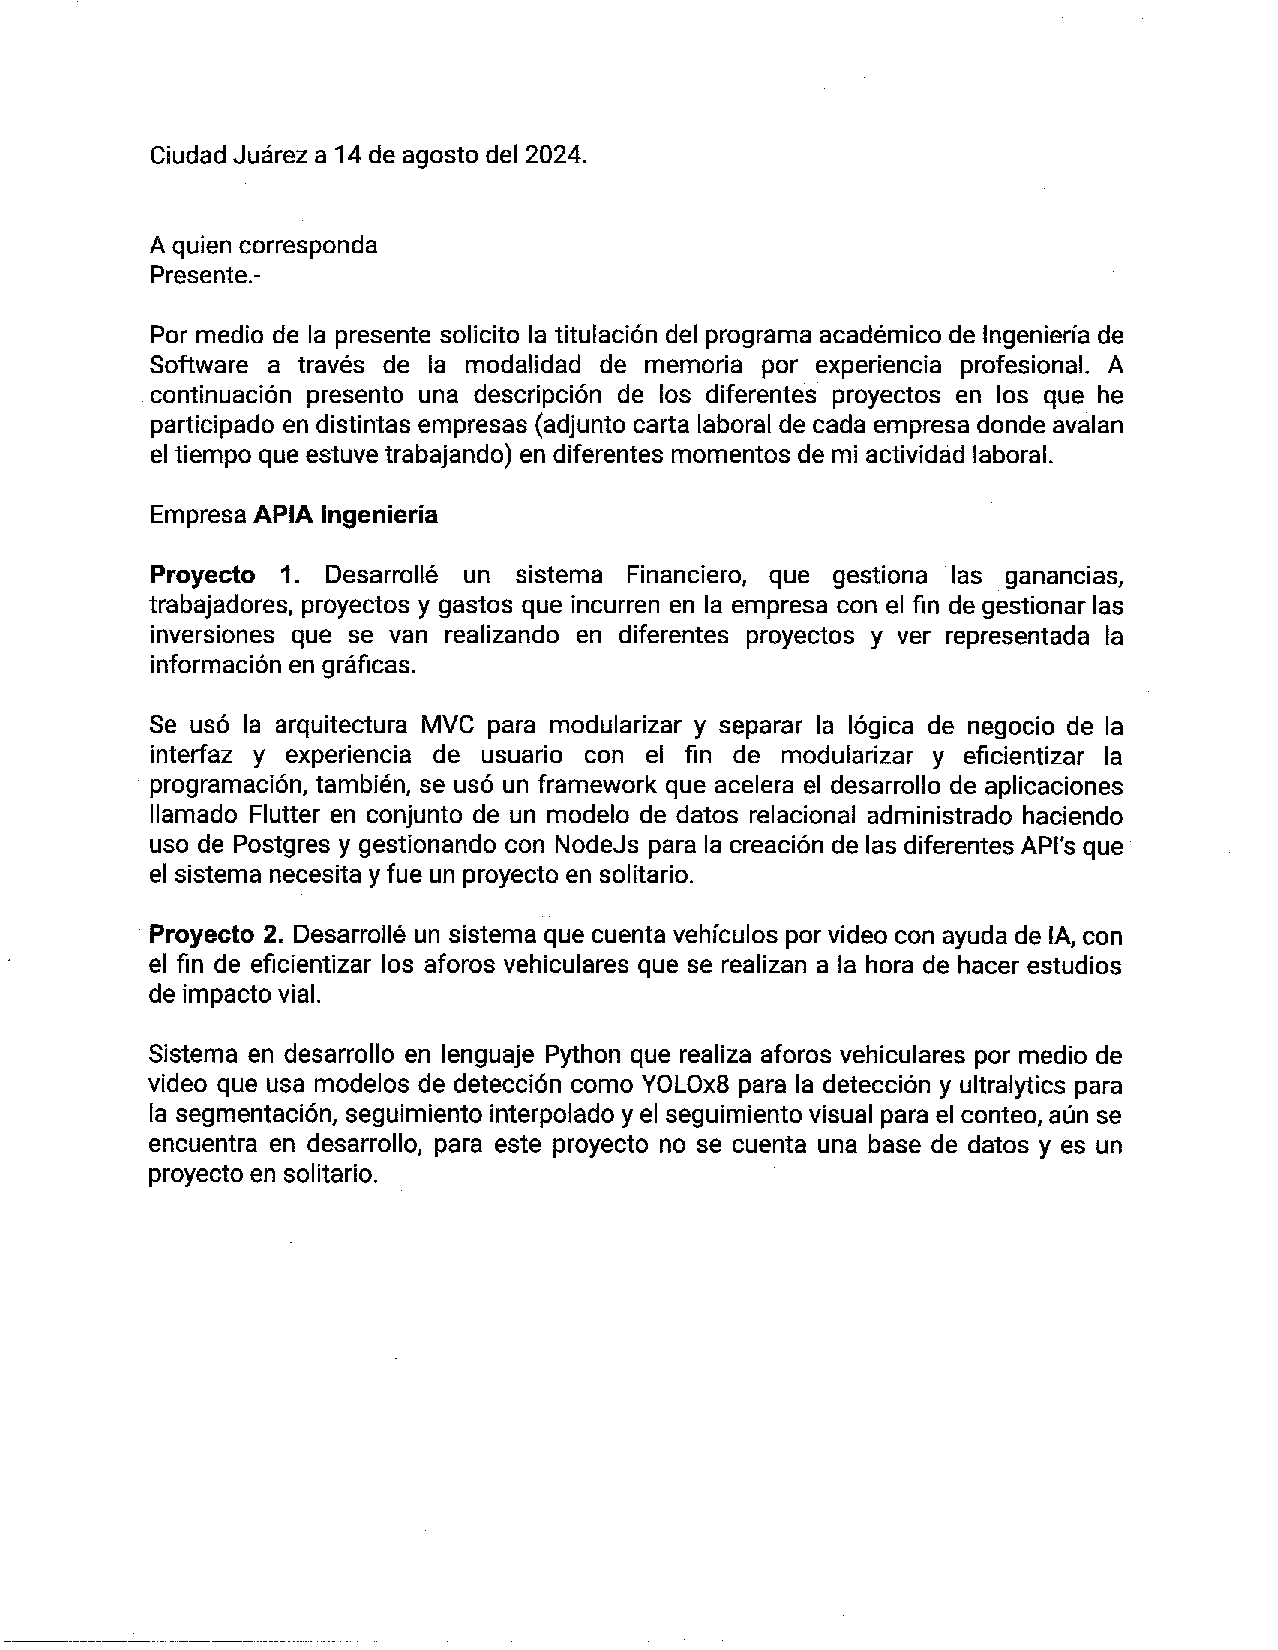
\includegraphics[scale=0.8]{Imagenes/Pdf/Carta1.pdf}

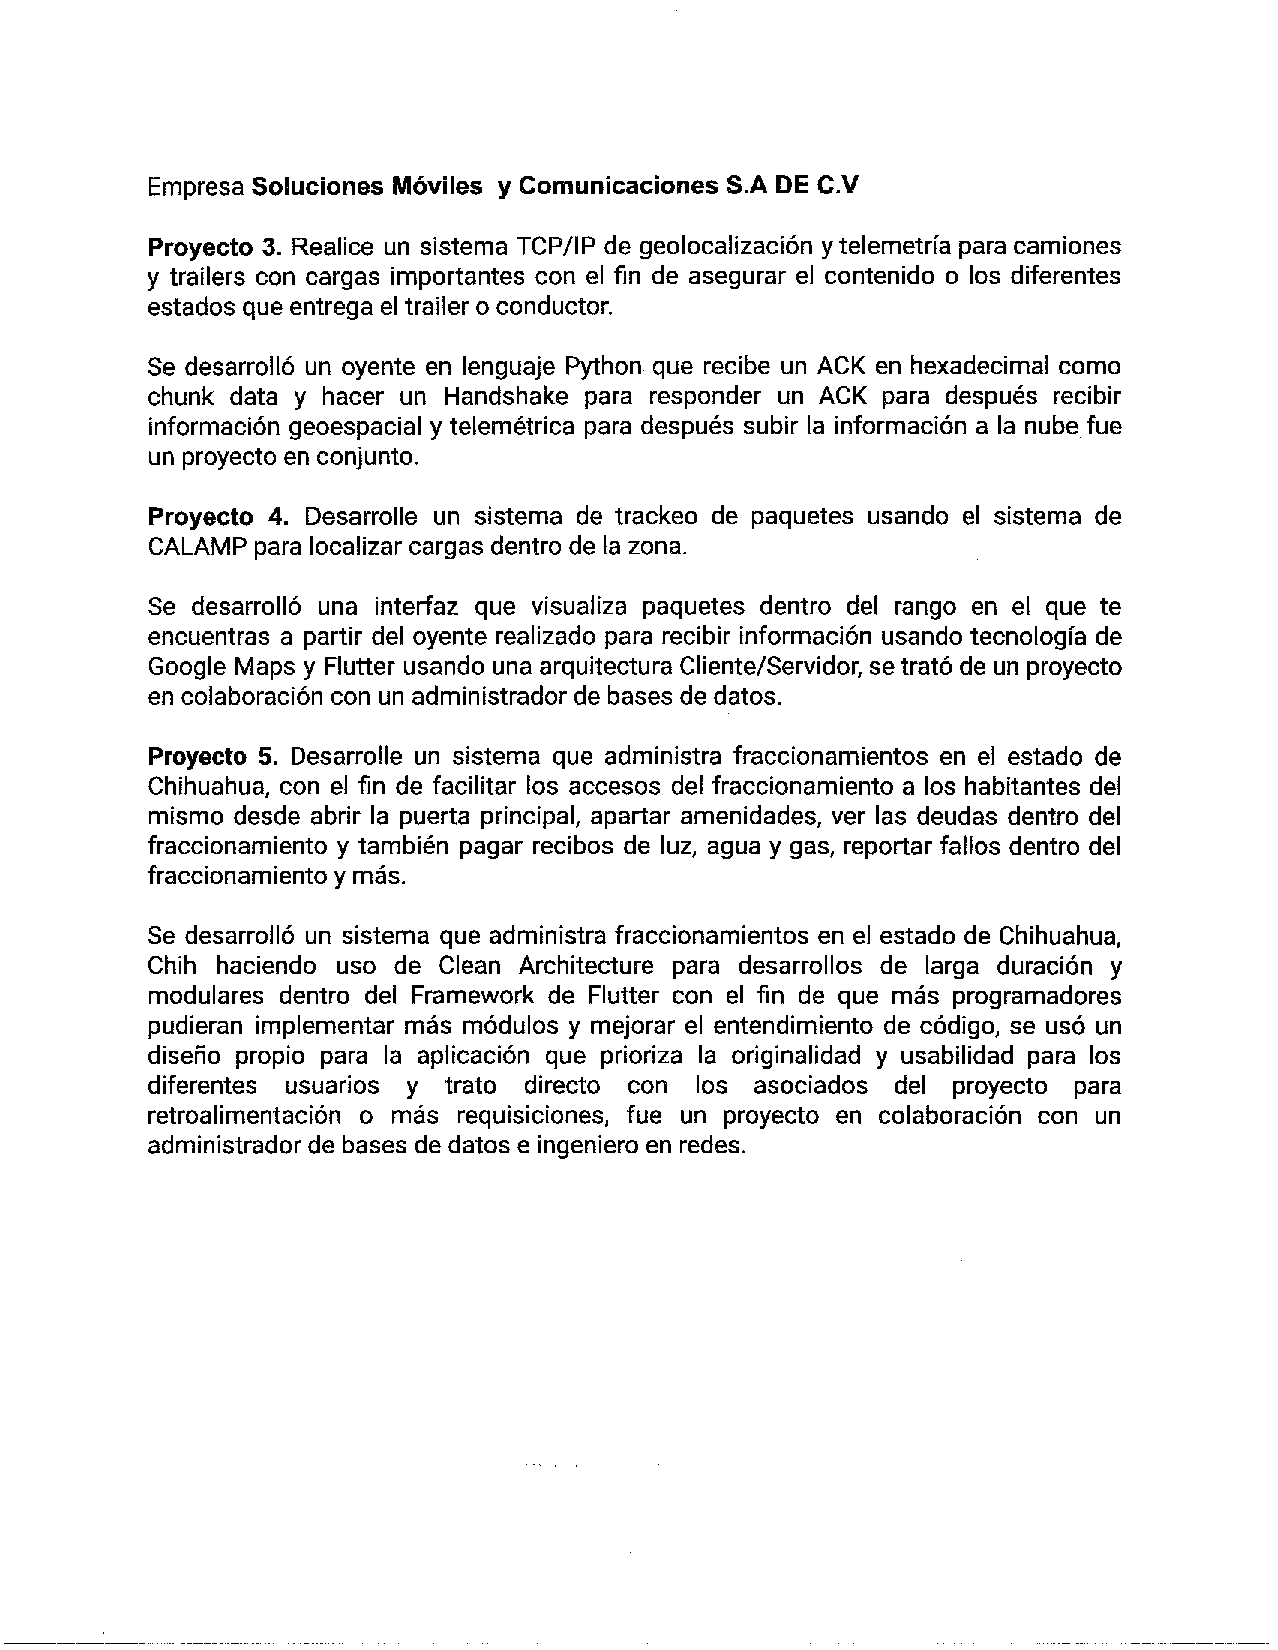
\includegraphics[scale=0.8]{Imagenes/Pdf/Carta2.pdf}

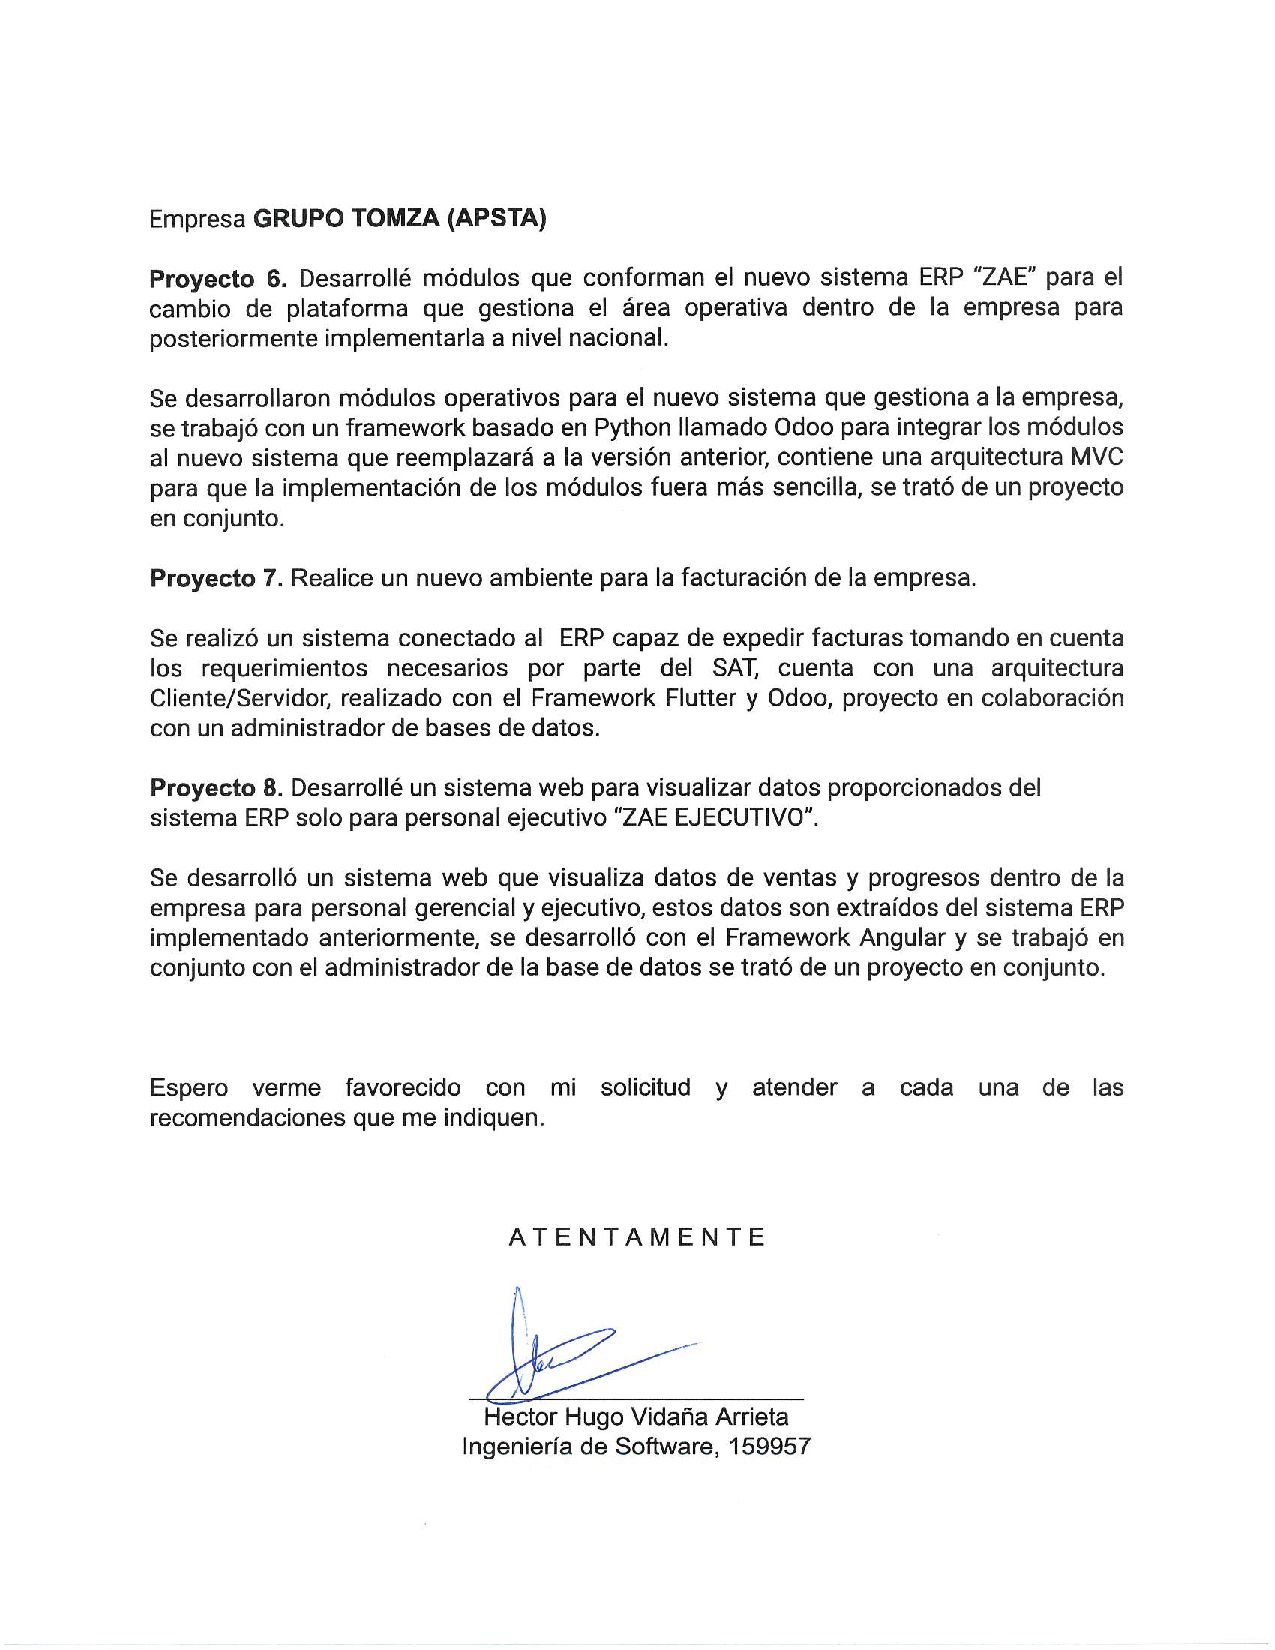
\includegraphics[scale=0.8]{Imagenes/Pdf/Carta3.pdf}

\end{center}

\end{document}  